\documentclass[a4paper,11pt]{jsarticle}

% 数式
\usepackage{amsmath,amsfonts}
\usepackage{amsthm}
\usepackage{bm}
\usepackage{mathtools}
\usepackage{amssymb}

% 表
\usepackage[utf8]{inputenc}
\usepackage{diagbox} % 斜線付きセルを作成するために必要
\usepackage{booktabs} % 表の罫線を美しくするために必要
\usepackage{hhline} % 水平罫線を制御するために必要

% 画像
\usepackage[dvipdfmx]{graphicx}
\usepackage{ascmac}
\usepackage{physics}
\usepackage{float} % 追加

% 図
\usepackage[dvipdfmx]{graphicx}
\usepackage{tikz} %図を描く
\usetikzlibrary{positioning, intersections, calc, arrows.meta,math} %tikzのlibrary

% ハイパーリンク
\usepackage[dvipdfm,
  colorlinks=false,
  bookmarks=true,
  bookmarksnumbered=false,
  pdfborder={0 0 0},
  bookmarkstype=toc]{hyperref}

% 式番号を章ごとにリセット
\numberwithin{equation}{section}

\begin{document}

\title{ゆらぎの定理}
\author{大上由人}
\date{\today}
\maketitle

\section{はじめに}
昔書いたゆらぎの定理RTAを書きなおす。\footnote{第1回ゆり京で発表しようと思っていたが結局没になった。}

\section{考える系}
\begin{figure}[H]
    \begin{center}
    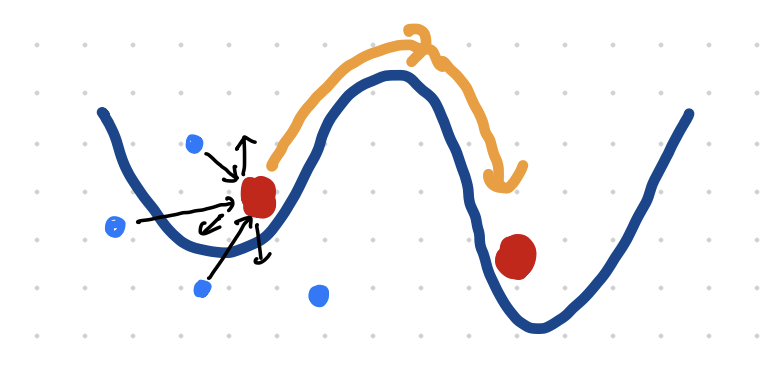
\includegraphics[width=80mm]{noneq.png}
    \end{center}
    \caption{考える系}
    \label{fig:one}
\end{figure}
まわりの熱浴によって系にゆらぎが生じような系を考える。例えば、水溶液中のコロイド粒子のようなものを考える。\\

\textbf{使う記号}
\begin{itemize}
    \item $w_{i}$: ある系の状態
    \item $p_i$: 状態$w_{i}$における系の確率分布
    \item $P_{w \to w'}$: 状態$w$から状態$w'$への遷移確率
    \item $\overline{w_{i}}$: 状態$w_{i}$の時間反転
    \item $P^{\dagger}_{\overline{w'}\to \overline{w}}$: 逆向き遷移(状態$\overline{w'}$から状態$\overline{w}$への遷移確率)
\end{itemize}

\begin{itembox}[l]{\textbf{平衡状態の性質}}
    平衡状態においては、
    \begin{align}
        p_{w}^{\text{eq}}P_{w\to w'} = p_{\bar{w'}}^{\text{eq}}P_{\bar{w'}\to \bar{w}}
    \end{align}
    が成り立つ。

\end{itembox}

\begin{itembox}[l]{\textbf{Def:熱(確率的)}}
    系から熱浴への確率的な熱の流れを、
    \begin{align}
        \hat{Q}_{w\to w'} = E_{w} - E_{w'} =\frac{1}{\beta}\ln \frac{P_{w\to w'}}{P_{\bar{w'}\to \bar{w}}}
    \end{align}
    と定義する。

\end{itembox}
$(\because)$(二つ目の等号)\\
\begin{align*}
    p_{w}^{\text{eq}} \propto e^{-\beta E_{w}}
\end{align*}
より、
\begin{align*}
    E_{w} - E_{w'} = -\frac{1}{\beta}\ln \frac{p_{w}^{\text{eq}}}{p_{w'}^{\text{eq}}}
\end{align*}
である。\footnote{若干ここ怪しい。}\\
いま、$p_{\bar{w'}}^{\text{eq}} = p_{w'}^{\text{eq}}$であることを用いると、
\begin{align*}
    E_{w} - E_{w'} = -\frac{1}{\beta}\ln \frac{p_{w}^{\text{eq}}}{p_{w'}^{\text{eq}}} = -\frac{1}{\beta}\ln \frac{P_{w\to w'}}{P_{\bar{w'}\to \bar{w}}}
\end{align*}
となる。\hfill\qedsymbol\\

\begin{itembox}[l]{\textbf{Def:Shanonエントロピー}}
    Shanonエントロピーを、
    \begin{align}
        S = -\sum_{i}p_{i}\ln p_{i}
    \end{align}
    と定義する。

\end{itembox}

\begin{itembox}[l]{\textbf{Def:エントロピー生成}}
    エントロピー生成を、
    \begin{align}
        \hat{\sigma} = \beta \hat{Q} + \Delta S
    \end{align}
    と定義する。

\end{itembox}

\begin{itembox}[l]{\textbf{Thm:DFT}}
    \begin{align}
        \frac{P(\hat{\sigma} = \Sigma)}{P(\hat{\sigma} = -\Sigma)} = e^{\Sigma}
    \end{align}
    が成り立つ。
\end{itembox}
\textbf{Prf}\\

\begin{itembox}[l]{\textbf{Thm:IFT}}
    \begin{align}
        \ev{e^{-\hat{\sigma}}}_{\text{eq}} = 1
    \end{align}
    が成り立つ。
\end{itembox}
\textbf{Prf}\\




\end{document}